\chapter{Design} \label{cha:Design}
Dette kapitlet tar for seg prosessen rundt designet av brukergrensesnittet til applikasjonen, resultatene som følge av designfasen og verktøyene som ble tatt i bruk under prosessen og utviklingen av grensesnittene.

\section{Verktøy}
\subsection{Coolors}
For å gjøre fargevalg for applikasjonens elementer enklere ble verktøyet Coolors fra coolors.co brukt \cite{BianchiCoolorsGenerator}. Verktøyet gjør det mulig å generere ulike fargepaletter helt fra bunnen av, men også med utgangspunkt i enkeltfarger. Verktøyet har også funksjonalitet for å hente ut fargene man finner på flere forskjellige formater, som blant annet hex \cite{ColorsHEX} og rgb \cite{ColorsRGB} som er veldig vanlige formater for å beskrive farger i utviklingsverdenen.

\subsection{Affinity Designer}
Under utvikling av applikasjonen viste det seg at det ble et behov for ikoner og illustrasjoner for bruk i applikasjonen som ikke lot seg lage i HTML eller CSS. For å unngå unødvendige kostnader ble valgt å utvikle disse elementene fra bunnen av framfor å bruke gratis dårlige ferdiglagde utgaver eller å betale for bra utgaver. For design av disse elementene ble verktøyet Affinity Designer \cite{AffinitySoftware} brukt. Affinity Deisgner er et designverktøy som brukes for å lage ulike grafikker, logoer, ikoner med mer og kan sammenlignes med det mer kjente Illustrator fra Adobe \cite{BransjeledendeIllustrator}. Affinity Designer ble i hovedsagt valgt fordi prosjektdeltakerne allerede hadde erfaring og tilgang til programvaren.

\subsection{Figma}
For å gjøre den programmatiske utviklingen av brukergrensesnittet mer effektivt ble det gjort et valg på at alle de ulike sidene av grensesnittet i applikasjonen først skulle tegnes i et design- og prototypeverktøy. Valget falt her på verktøyet Figma \cite{Figma:Tool.}. Andre verktøy som Adobe XD \cite{AdobeTool} og Balsamiq \cite{BalsamiqBalsamiq} ble også vurdert. Her ble det fordelaktig å velge Figma foran både Adobe XD og Balsamiq. Adobe XD og Figma er ganske like i funksjonalitet, men på grunn av tidligere erfaring i Figma ble Adobe XD valgt bort. Begge prosjektdeltakerne hadde erfaring med bruk av både Balsamiq og Figma. Det ble valgt å ikke bruke Balsamiq ettersom at det ikke tilbyr den ønskede funksjonaliteten da det er et mye enklere og mer primitivt verktøy.
\newline

\noindent
Figma gjør det mulig å designe fullstendige brukergrensesnitt som kan gjøres om til enkle prototyper for testing av basisfunksjonalitet. Figma er også laget for at det skal være enkelt å samarbeide og tilbyr funksjonalitet for å designe elementer sammen i sanntid over nettet.

\section{Resultater}
\subsection{Fargevalg}
Valget av fargepaletten i applikasjonen falt på en applikasjon med mørkt tema. Både fordi at det er populært i dagens applikasjonsmarked, men også fordi det kan føre til at applikasjonen på mobiler med OLED-skjermer \cite{OLEDOLED-Info} vil bruke mindre strøm under operasjon \cite{WhatEnerlytics}. Dette er viktig ettersom at applikasjonen skal kunne brukes lenge uten tilgang på strøm mens man går oppsynstur. Bakgrunnsfargen (hovedfargen) i applikasjonen er en mørk marineblå farge. Denne blir komplementert med en dus grønnfarge som blir brukt på knapper og enkelte andre elementer. Fargen på tekst gjennom nærmest hele applikasjonen er hvit. Fargevalget har resultert i en applikasjon hvor det er god kontrast mellom ulike elementer. Det er også god kontrast mellom de ulike elementene og tilhørende tekst. For å sørge for at applikasjonen er tilgjengelighet for personer med de vanligste formene for fargeblindhet brukte vi nettleserutvidelsen-utvidelsen Colorblinding \cite{LeonardoCardoso/Colorblinding:See.} under testing av ulike fargekombinasjoner.

\begin{figure}[H]
\centering
\captionsetup{width=.8\linewidth}
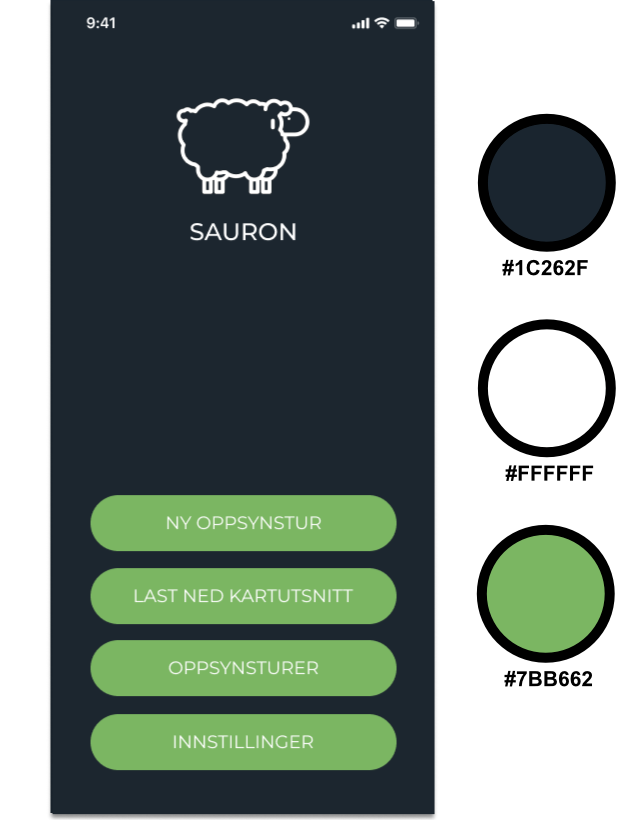
\includegraphics[scale=0.4]{Figurer/Bilder/valg-av-farger.png}
\caption{Illustrasjon av hovedmenyen i applikasjonen samt de ulike fargene brukt og deres tilhørende hex-verdier.}
\label{fig:valg-av-farger}
\end{figure}

\subsection{Nedlasting av kartutsnitt}
For å laste ned kartutsnitt kan man navigere seg til oversikten over nedlastede kartutsnitt fra hovedmenyen (figur \ref{fig:valg-av-farger}) ved å trykke på \enquote{Last ned kartutsnitt}-knappen. Oversikten viser alle nedlastede kartutsnitt, hvor mye plass kartutsnittene tar på mobilen og når de ble lastet ned.

\begin{figure}[H]
\centering
\captionsetup{width=.8\linewidth}
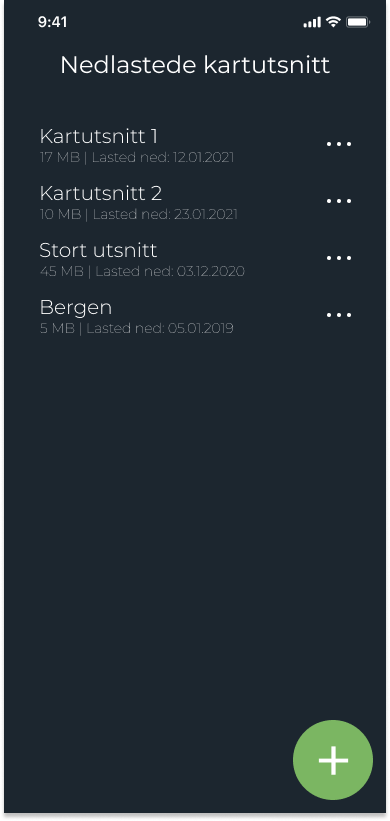
\includegraphics[scale=0.4]{Figurer/Figma/Frame 4 - Nedlastede kartutsnitt.png}
\caption{Prototypedesign av side for oversikt over nedlastede kartutsnitt.}
\label{fig:figma-nedlastede-kartutsnitt}
\end{figure}
\noindent
De tre prikkene på høyresiden av hvert nedlastede kartutsnitt kan trykkes på for å åpne en valgmeny (figur \ref{fig:figma-nedlastede-kartutsnitt-med-apen-meny}). Valgmenyen tilbyr fire valg. Man kan trykke på \enquote{Oppdater} for å oppdatere et valgt kartutsnitt og dermed laste ned kartutsnittet på nytt igjen. Ved å trykke på \enquote{Gi nytt navn} kan man gi kartutsnittet et nytt navn framfor å bruke det autogenererte navnet gitt av applikasjonen. Dette kan være nytting om man har flere forskjellige kartutsnitt man ønsker å holde kontroll på. \enquote{Slett}-knappen sletter et valgt kartutsnitt og \enquote{Avbryt}-knappen lukker valgmenyen.
\begin{figure}[H]
\centering
\captionsetup{width=.8\linewidth}
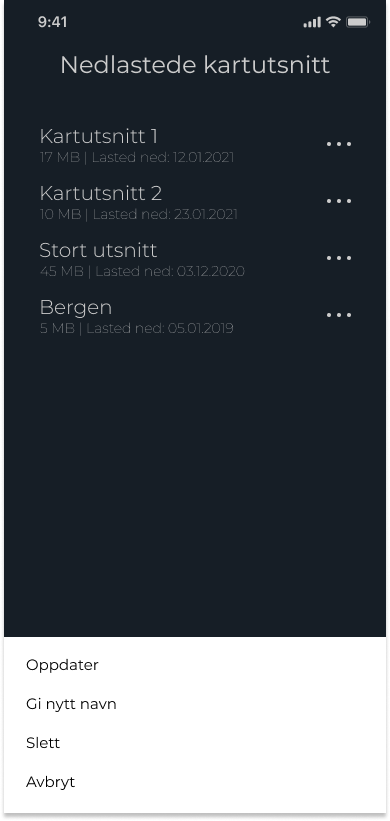
\includegraphics[scale=0.4]{Figurer/Figma/Frame 5 - Nedlastede kartutsnitt meny.png}
\caption{Prototypedesign av side for oversikt over nedlastede kartutsnitt med åpen valgmeny.}
\label{fig:figma-nedlastede-kartutsnitt-med-apen-meny}
\end{figure}
\noindent
Om man trykker på den grønne knappen med et pluss-tegn nede i høyre hjørne på \enquote{Nedlastede kartutsnitt}-siden, vil det navigeres til siden hvor man kan laste ned nye kartutsnitt (figur \ref{fig:figma-laste-ned-kartutsnitt}). Ved å flytte og zoome på kartet slik at det ønskede kartutsnittet kommer innenfor det markerte rektangelet kan man selv velge hvor stort et kartutsnitt skal være. Når man har funnet området på kartet man ønsker å lage et kartutsnitt av trykker man på \enquote{Last ned}-knappen. Ved å trykke på \enquote{Avbryt}-knappen vil man bli tatt tilbake til oversikten over nedlastede kartutsnitt.
\begin{figure}[H]
\centering
\captionsetup{width=.8\linewidth}
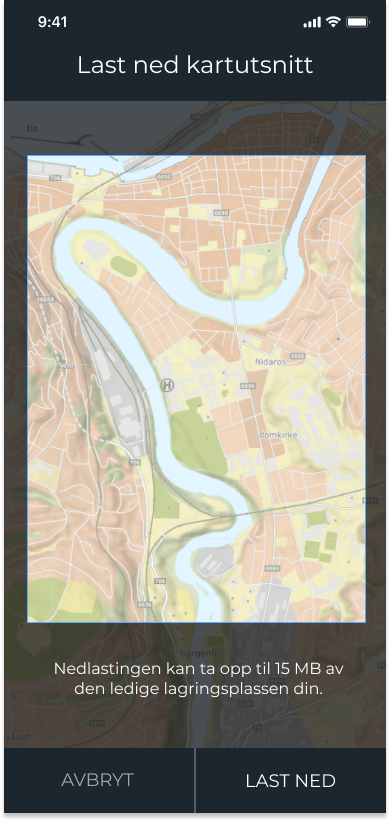
\includegraphics[scale=0.4]{Figurer/Figma/Frame 3 - Last ned kartutsnitt.png}
\caption{Prototypedesign av side for å laste ned nye kartutsnitt.}
\label{fig:figma-laste-ned-kartutsnitt}
\end{figure}

\subsection{Ny oppsynstur}
\subsubsection{Registrering av informasjon}
For å registrere en ny oppsynstur kan man trykke på \enquote{Ny oppsynstur}-knappen på hovedmenyen (figur \ref{fig:valg-av-farger}). Da blir man først tatt til \enquote{Ny oppsynstur}-siden (figur \ref{fig:figma-info-ny-oppsynstur}). Her skal man registrere navnet på deltagerne som er med på oppsynsturen, samt at man kan legge til en beskrivelse for turens formål og baktanke. Når dette er gjort kan man trykke på \enquote{Start oppsynstur}-knappen for å starte selve oppsynsturen. Brukeren vil da bli tatt til kartsiden som er hovedsiden under en oppsynstur.
\begin{figure}[H]
\centering
\captionsetup{width=.8\linewidth}
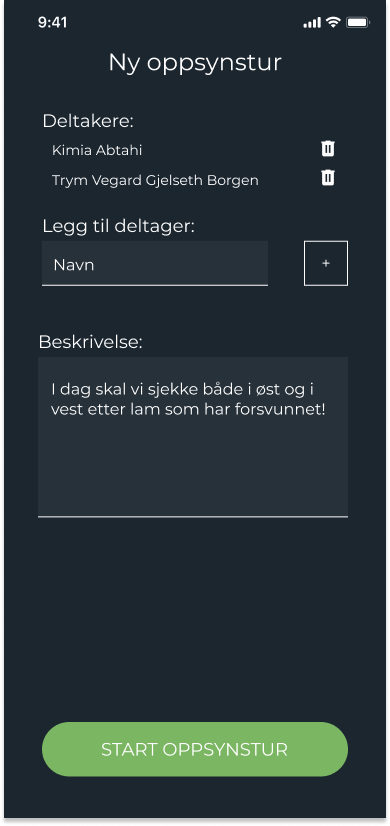
\includegraphics[scale=0.4]{Figurer/Figma/Frame 2 - Ny oppsynstur.png}
\caption{Prototypedesign av side for å registrere informasjon til en ny oppsynstur.}
\label{fig:figma-info-ny-oppsynstur}
\end{figure}

\subsubsection{Kart}
Kartsiden (figur \ref{fig:figma-kart}) i applikasjonen er, som nevnt tidligere, siden som blir mest brukt under en oppsynstur. Kartsiden viser ved hjelp av en blå sirkel hvor man befinner seg på kartet, mens den blå streken viser hvor man har gått.
\begin{figure}[H]
\centering
\captionsetup{width=.8\linewidth}
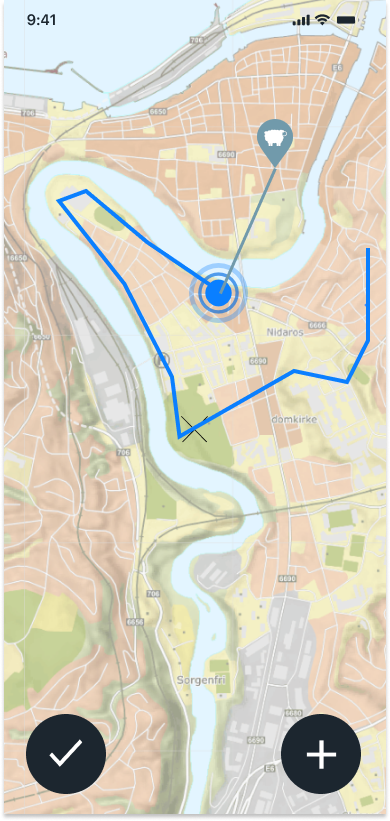
\includegraphics[scale=0.4]{Figurer/Figma/Frame 2.1 - Oppsynstur-kart.png}
\caption{Prototypedesign av side for kart.}
\label{fig:figma-kart}
\end{figure}

\subsubsection{Meny i kart}
Ved å trykke på pluss-knappen nede i høyre hjørne åpnes valgmenyen for å legge til en ny registrering (figur \ref{fig:figma-kart-apen-meny}). Her kan man velge mellom (fra øverst til nederst) å legge til en registrering for en observasjon av en saueflokk, rovdyr, en eller flere døde sauer og en eller flere skadde sauer. Når en registrering har blitt fullført legges det til to ny elementer på kartsiden:
\begin{itemize}
    \item Et merke som viser hvilken type registrering som har blitt utført (Død sau, rovdyr etc.). Dette merket blir da plassert på posisjonen hvor observasjonen ble gjort.
    \item En linje som peker fra hvor observasjonen ble gjort fra og til merket.
\end{itemize}

\noindent
På den måten kan brukeren i etterkant av en oppsyntur vite både hvor eventuelle sauer har blitt observert i tillegg til hvor de ble observert fra. 

\begin{figure}[H]
\centering
\captionsetup{width=.8\linewidth}
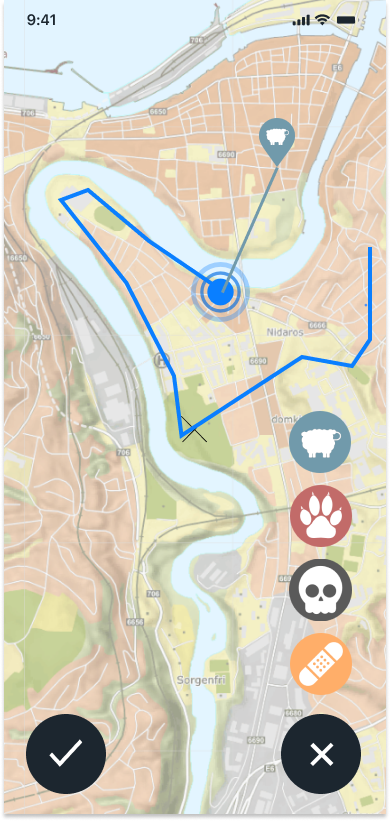
\includegraphics[scale=0.4]{Figurer/Figma/Frame 2.1 - Oppsynstur-kart-apen-meny.png}
\caption{Prototypedesign av side for kart med åpen valgmeny.}
\label{fig:figma-kart-apen-meny}
\end{figure}

\subsection{Fullføre oppsynstur}
For å fullføre en oppsynstur trykkes det på fullfør-knappen nede i venstre hjørne på kartsiden (figur \ref{fig:figma-kart}). Ved å gjøre dette vil applikasjonen navigere til \enquote{Oppsummering}-siden (figur \ref{fig:figma-oppsummering}). Oppsummeringssiden viser generell informasjon om turen, samt hvor brukeren har gått og hvilke observasjoner som har blitt gjort. Her er det også mulig å legge til en kommentar før det trykkes fullfør og oppsynsturen blir lagret.
\begin{figure}[H]
\centering
\captionsetup{width=.8\linewidth}
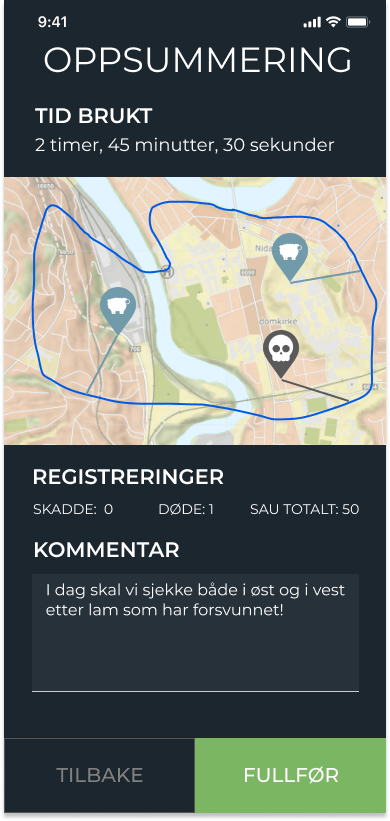
\includegraphics[scale=0.4]{Figurer/Figma/Frame 2.3 - Oppsummering oppsynstur.png}
\caption{Prototypedesign av side for oppsummering av en oppsynstur.}
\label{fig:figma-oppsummering}
\end{figure}

\subsection{Legge til en registrering}
\subsubsection{Registrering av sau} 
\label{subsubsec:registrering av sau}
Grensesnittet for registrering av sau ble nesten ferdig utformet i fordypningsprosjektet og kan leses om i sin helehet der \cite{Abtahi2020TilsynBeite}. Det eneste som har blitt lagt til grensesnittet for registrering av sau siden da er funksjonalitet for å legge til øremerker. Figur \ref{fig:figma-legge-til-oremerker} viser den nye siden for registrering av øremerker. Listen er en flervalgsliste som inneholder fargen på merket og navnet på bonden som øremerkene tilhører.
\begin{figure}[H]
\centering
\captionsetup{width=.8\linewidth}
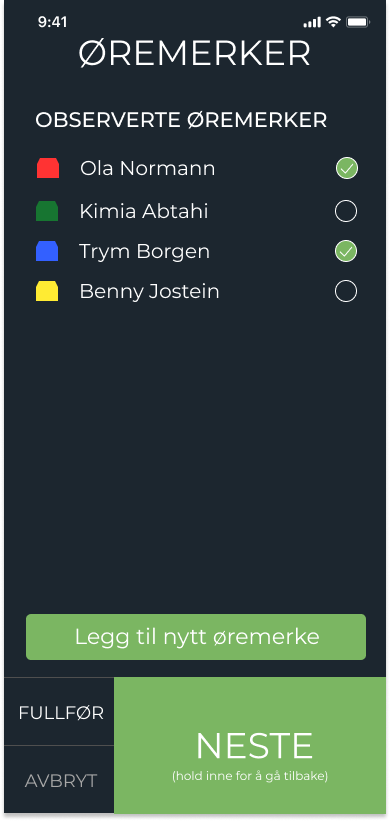
\includegraphics[scale=0.4]{Figurer/Figma/Frame 2.2.2 - oremerker.png}
\caption{Prototypedesign av side for å legge til et øremerker i en registrering.}
\label{fig:figma-legge-til-oremerker}
\end{figure}
\noindent
For å legge til et nytt øremerke i lista trykker man på \enquote{Legg til nytt øremerke}-knappen (figur \ref{fig:figma-legge-til-oremerker}). Det vil åpne et annet grensesnitt hvor man kan registrere et nytt øremerke (figur \ref{fig:figma-registrere-nytt-oremerke}). I \enquote{Eier}-feltet skriver mann inn navnet på bonden som eier sauene som bærer det nye øremerket. Fargen(e) på merket legges til i grensesnittet under. Mattilsynets regler for øremerker \cite{Mattilsynet2013remerkingSmafe} sier at alle farer er tillatt, med unntak av hvit, lilla og lakserød. Etter en undersøkelse av flere kilder \cite{remerker, GolSA, NannestadGeit} for beitelag og saumerker virker det som om de fleste øremerker består av enten 1 eller 2 farger. Den foreslåtte løsningen tillatter at det legges til maks 2 farger per øremerke. Fargevelgeren gjør det mulig å velge mellom alle mulige fargekombinasjoner som måtte være ønskelig for brukeren.
\begin{figure}[H]
\centering
\captionsetup{width=.8\linewidth}
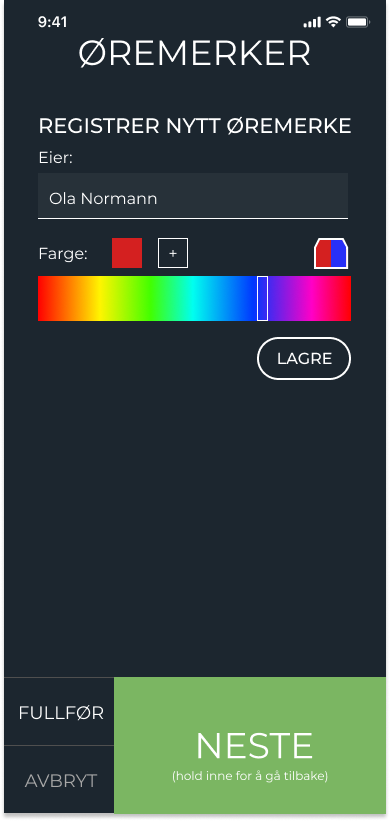
\includegraphics[scale=0.4]{Figurer/Figma/Frame 2.2.2 - lag-oremerke.png}
\caption{Prototypedesign av side for å registrere et nytt øremerke.}
\label{fig:figma-registrere-nytt-oremerke}
\end{figure}
\noindent
Oppsummeringssiden (figur \ref{fig:figma-sau-oppsummering}) for registrering av sau har også blitt oppdatert for å vise hvilke øremerker som har blitt valgt under en registrering. Ellers er den identisk med oppsummeringssiden som ble laget under fordypningsprosjektet.

\begin{figure}[H]
\centering
\captionsetup{width=.8\linewidth}
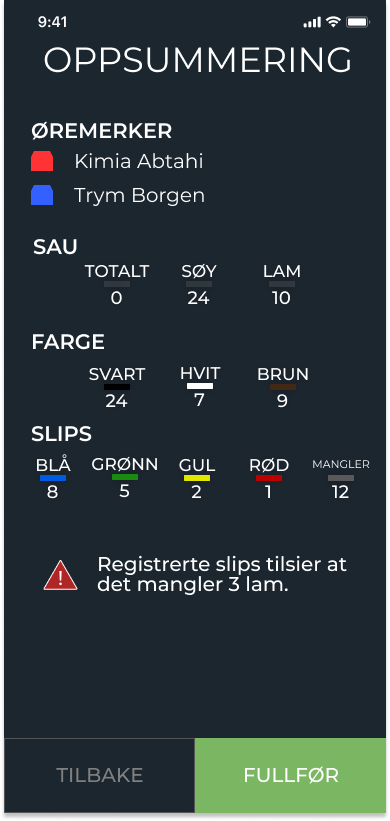
\includegraphics[scale=0.4]{Figurer/Figma/Frame 2.2.5 - Oppsummering.png}
\caption{Prototypedesign av side for oppsummering for registrering av sau.}
\label{fig:figma-sau-oppsummering}
\end{figure}

\subsubsection{Registrering av rovdyr}
For å registrere et rovdyr trykker man på det røde ikonet i valgmenyen med et poteavtrykk (figur \ref{fig:figma-kart-apen-meny}). Herfra blir man tatt til registreringssiden for rovdyr (figur \ref{fig:figma-registrer-rovdyr}). Rovdyrene man kan legge til er forhåndsbestemt og kan enkelt velges fra nedtrekkslisten. Valget av rovdyr begrunnes i underkapittel \ref{sub:rovdyr} \nameref{sub:rovdyr}. I tillegg til dette kan man legge til en kommentar om man ønsker. Man kan fullføre regitereringen ved å trykke på \enquote{Fullfør}-knappen. Registreringen kan også avbrytes ved å trykke på \enquote{Tilbake}-knappen som tar brukeren tilbake til kartsiden.
\begin{figure}[H]
\centering
\captionsetup{width=.8\linewidth}
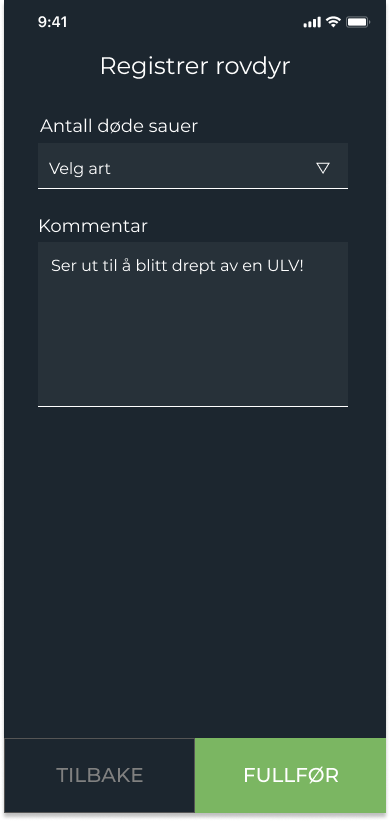
\includegraphics[scale=0.4]{Figurer/Figma/Frame 2.2c.1 - Registrer rovdyr.png}
\caption{Prototypedesign av side for registrering av rovdyr.}
\label{fig:figma-registrer-rovdyr}
\end{figure}

\subsubsection{Registrering av død sau}
For å registrere død sau trykker man på den mørkegrå knappen med et dødninghode i valgmenyen på kartsiden (figur \ref{fig:figma-kart-apen-meny}). Deretter blir man tatt til registreringssiden for døde sauer (figur \ref{fig:figma-registrer-dode-sauer}). Antallet døde sauer man finner på en lokasjon registreres under feltet \enquote{Antall døde sauer}. Man kan også legge til en kommentar om ønskelig. I følge Statsforvalteren skal det ved mistanke om skade på sau som følge av rovdyr tas bilde av kadaveret som knyttes til GPS-koordinater \cite[~s.19]{StatsforvaltereniInnlandet2020InformasjonInnlandet}. Denne informasjonen blir brukt som grunnlag når det søkes om erstatning for tap av sau \cite{2014ForskriftRovvilt, MiljdirektoratetErstatningRovvilt}. Det er derfor lagd design for funksjonalitet som lar brukeren legge til et eller flere bilder som blir lagret sammen med registreringen. Etter at ønsket informasjon er fylt ut kan man trykke på \enquote{Fullfør}-knappen for å lagre registreringen og gå tilbake til kartsiden. Hvis man ikke ønsker å lagre registreringen kan man trykke på \enquote{Tilbake}-knappen.
\begin{figure}[H]
\centering
\captionsetup{width=.8\linewidth}
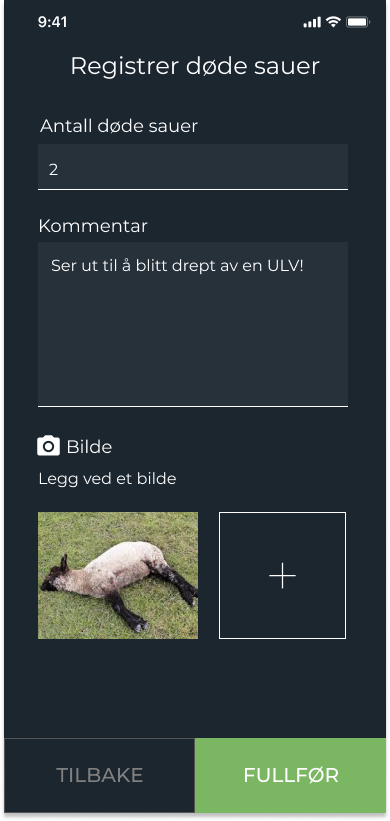
\includegraphics[scale=0.4]{Figurer/Figma/Frame 2.2b.1 - Registrer-dode-sauer.png}
\caption{Prototypedesign av side for registrering av døde sauer.}
\label{fig:figma-registrer-dode-sauer}
\end{figure}

\subsubsection{Registrering av skadet sau}
For å registrere skadet sau trykker man på den gule knappen med et plaster i valgmenyen på kartsiden (figur \ref{fig:figma-kart-apen-meny}). Herfra blir man tatt til siden for registrering av skadet sau (figur \ref{fig:figma-registrer-skadd-sau}). Antall skadde sauer registreres under feltet \enquote{Antall skadde sauer}. Det er også mulig å legge ved en eventuell kommentar. Når registreringen er fullført trykker man på \enquote{Fullfør}-knappen for å lagre registreringen og gå tilbake til kartsiden. Hvis man ønsker å forkaste registreringen kan man trykke på \enquote{Tilbake}-knappen for å gå tilbake til kartsiden uten å lagre.
\begin{figure}[H]
\centering
\captionsetup{width=.8\linewidth}
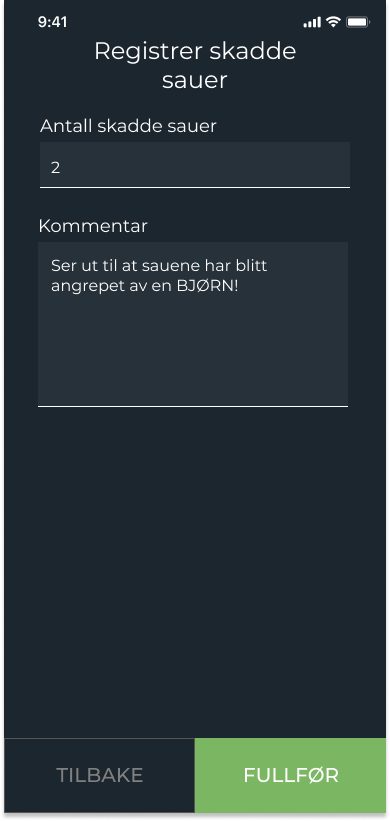
\includegraphics[scale=0.4  ]{Figurer/Figma/Frame 2.2a.1 - Registrer-skadde-sauer.png}
\caption{Prototypedesign av side for registrering av skadd sauer.}
\label{fig:figma-registrer-skadd-sau}
\end{figure}

\subsection{Lagrede oppsynsturer}
\subsubsection{Liste over lagrede oppsynsturer}
Fra hovedmenyen (figur \ref{fig:valg-av-farger}) kan man navigere seg til en liste over alle lagrede oppsynsturer (figur \ref{fig:figma-oppsynsturer-liste}) ved å trykke på \enquote{Oppsynsturer}-knappen. Hvert element i lista viser én lagret oppsynstur og litt generell informasjon om turen, som hvem som registrerte oppsynsturen, hvor lang tid det tok og hvilken dato den ble utført på. Symbolene nederst i hvert element viser (fra venstre) hvor mange sau som har blitt registrert totalt, hvor mange skadde sau som har blitt registrert, hvor mange døde sau som har blitt registrert og hvor mange rovdyr som har blitt registert.

\begin{figure}[H]
\centering
\captionsetup{width=.8\linewidth}
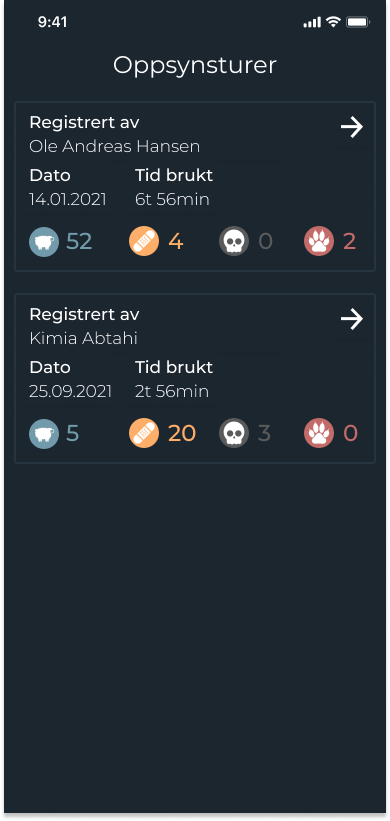
\includegraphics[scale=0.4]{Figurer/Figma/Frame 6 - Oppsynsturer.png}
\caption{Prototypedesign av side for lagrede oppsynsturer.}
\label{fig:figma-oppsynsturer-liste}
\end{figure}

\subsubsection{Oppsummering av en enkelt oppsynstur}
Ved å trykke på pila i et element i lista over oppsynsturer (figur \ref{fig:figma-oppsynsturer-liste}) blir man tatt til siden som viser detaljert informasjon om den valgte oppsynsturen (figur \ref{fig:figma-lagret-oppsynstur}). Siden viser ruta man har gått på kartet, samt alle registreringer som har blitt gjort og hvor de ble gjort fra. Under kartet er fire ekspanderbare elementer som kan åpnes og lukkes for å vise de forskjellige registreringene som har blitt gjort under hver av de fire kategoriene. Ikonet med tallet på siden viser det totale antallet sau, skadde sau, døde sau eller rovdyr som har blitt registrert under kategorien. Ved å trykke på pila til høyre i boksen ekspanderes lista, og alle registreringer som er gjort innenfor den valgte kategorien vises med all registert informasjon.
\begin{figure}[H]
\centering
\captionsetup{width=.8\linewidth}
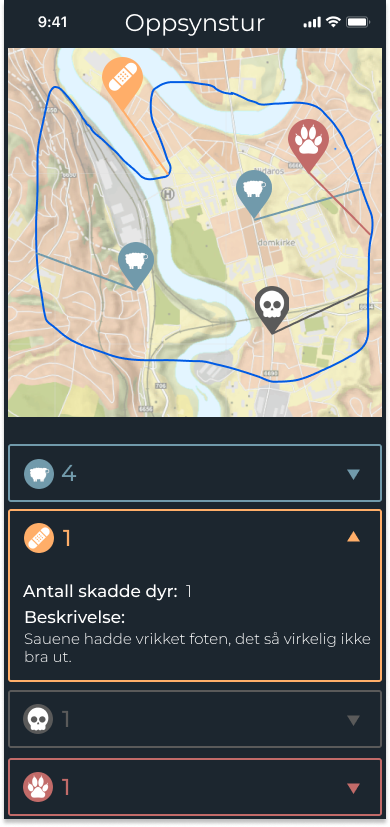
\includegraphics[scale=0.4]{Figurer/Figma/Frame 7 - Oppsynstur-oppsummering.png}
\caption{Prototypedesign av side for oppsummering av en lagret oppsynstur som viser registreringer for skadet sau.}
\label{fig:figma-lagret-oppsynstur}
\end{figure}
\noindent
Ettersom at de forskjellige kategoriene inneholder forskjellig informasjon vil elementene inne i de ekspanderbare boksene være ulike fra kategori til kategori. Figur \ref{fig:figma-lagret-oppsynstur2} viser hvordan informasjonen inne i den ekspanderte boksen for registrering av en saueflokk ser ut.
\begin{figure}[H]
\centering
\captionsetup{width=.8\linewidth}
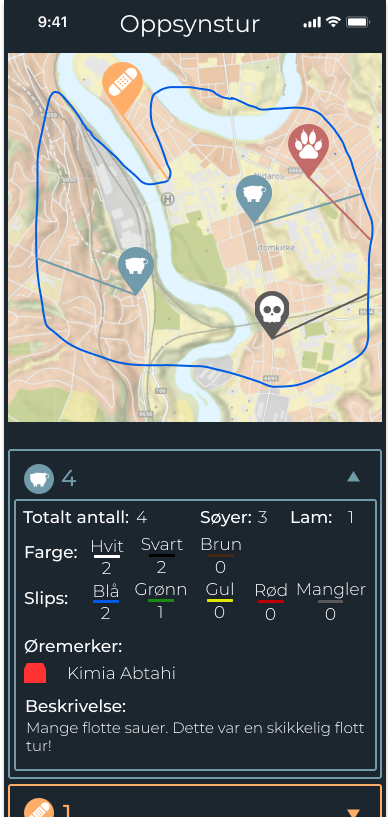
\includegraphics[scale=0.4]{Figurer/Figma/Frame 7 - Oppsynstur-oppsummering2.png}
\caption{Prototypedesign av side for oppsummering av en lagret oppsynstur som viser registreringer for en saueflokk.}
\label{fig:figma-lagret-oppsynstur2}
\end{figure}